%%%  default
\documentclass[10pt, compress]{beamer}


\usetheme{mnuigD}
\usepackage{tikz}
\usepackage{booktabs}
%\usepackage{cite}
\bibliographystyle{apalike}
\usepackage[export]{adjustbox}
\usepackage{subfig}
%\usepackage[scale=2]{ccicons}

%\usemintedstyle{trac}
\usepackage{grffile} %for underscores in file names

\title{Automating riboSeed assembly assessment }
\subtitle{Lab Meeting}
\date{\footnotesize{\today}}
\author{\\ \\ \\ \\\large{Nick Waters}}
\institute{% \includegraphics[height=1cm]{../stock_logos/NUI_Galway_BrandMark_A_K.eps}
\includegraphics[height=.9cm, trim=2 -.2cm 0cm .4cm]{../stock_logos/trimmed_jhi.png}
  Department of Microbiology\\
School of Natural Sciences\\
National University of Ireland Galway}

%%%%% %%%%% %%%%% %%% %%%%  for pretty headers with pictures
\addtobeamertemplate{frametitle}{}{%
\begin{tikzpicture}[remember picture,overlay]
\node[anchor=north east,yshift=2pt] at (current page.north east) {
\includegraphics[height=0.8cm]{../stock_logos/nuig_rounded.png}  \hspace*{.05cm} 
\includegraphics[height=.794cm, trim= 0cm 0.0cm 0.0cm 0cm]{../stock_logos/jhi_rounded.png}};
\end{tikzpicture}}


\begin{document}
\maketitle

%\maketitle
% \section{Outline}

% \begin{frame}[fragile]
%   \frametitle{}
%   \begin{itemize}%[<+- | alert@+>]
%   \item De Bruijn Graphs and short read assembly
%   \item Shortcoming of Short Read Assembly
%     \item Genome Finishing Strategies
%   \item riboSeed
%   \item Challenges
%   \end{itemize}
% \end{frame}

\section{Problem}



\begin{frame}[fragile]
  \frametitle{Problem}
\begin{table}[]
\centering
\caption{Runs of riboSeed by manuscript section}
\label{my-label}
\begin{tabular}{lll}
 & runs & repetitions \\
background & 8 & 8 \\
simulated genome & 6 & 1 \\
simulated reads & 12 & 4 \\
GAGE-B & 16 &  \\
other & 10 &
\end{tabular}
\end{table}
\end{frame}


\begin{frame}[fragile]
  \frametitle{Problem: Sample Result Visualization}
  \centering
  \hspace*{-1.7cm}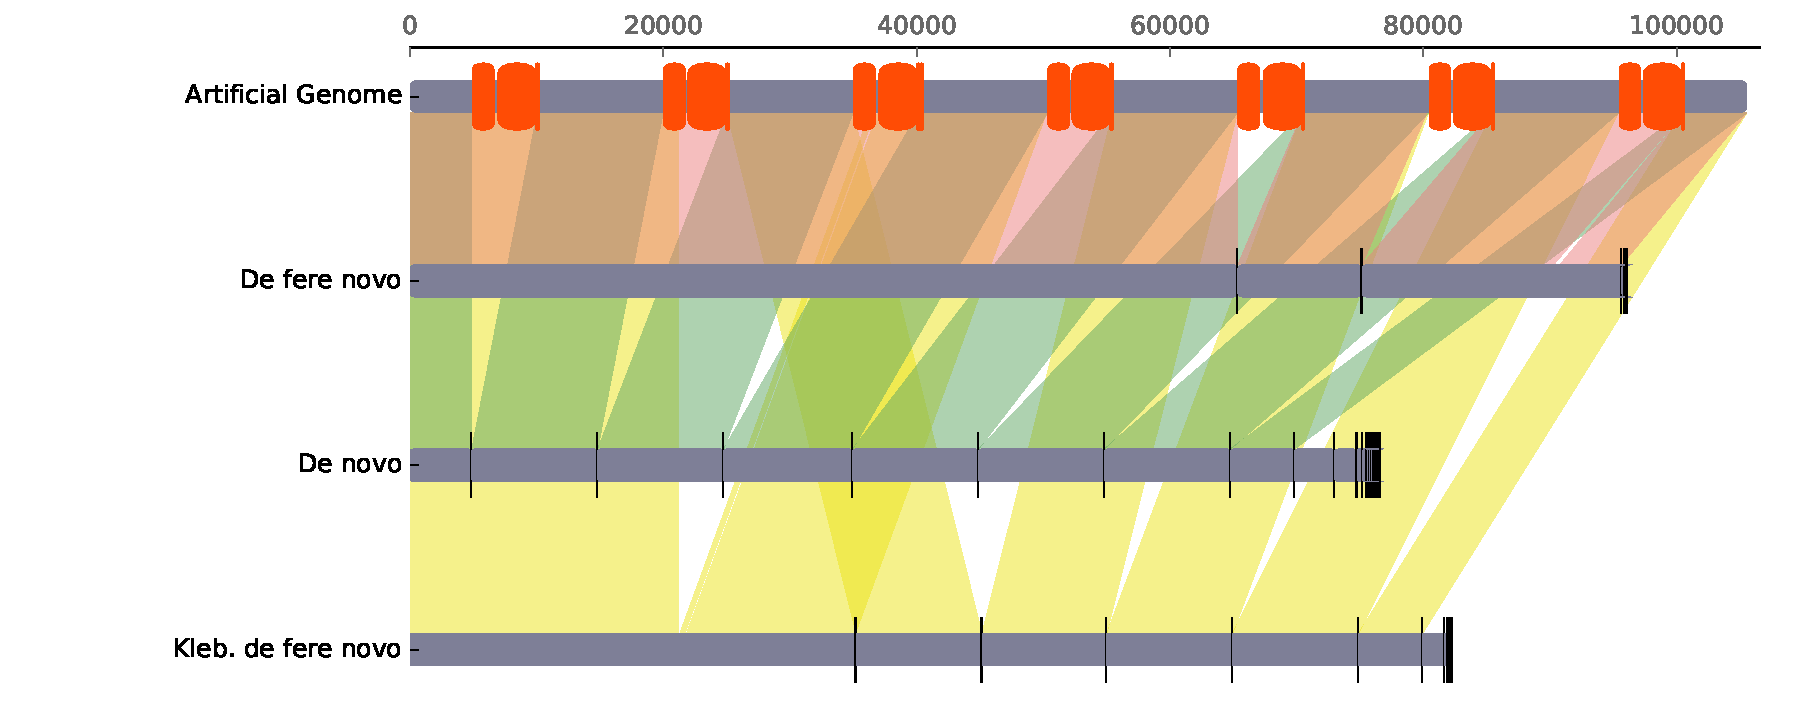
\includegraphics[width=1.25\textwidth]{~/GitHub/FB/Ecoli_comparative_genomics/doc/presentations/MyNUIG(mnuigtheme)/frequentFigs/PrettyMauve.pdf}

\end{frame}


\section{Solution 1: Full length Matches}



\begin{frame}[fragile]
  \frametitle{Solution 1}
  \begin{itemize}
  \item Annotate and extract rDNAs and flanking regions from reference and assemblies
  \item Use BLAST or Mummer to find best reciprocal matches
  \end{itemize}


\end{frame}

\begin{frame}[fragile]
  \frametitle{Solution 1: Results}
  Accurately characterized true positives
  \centering
  \hspace*{-1.7cm}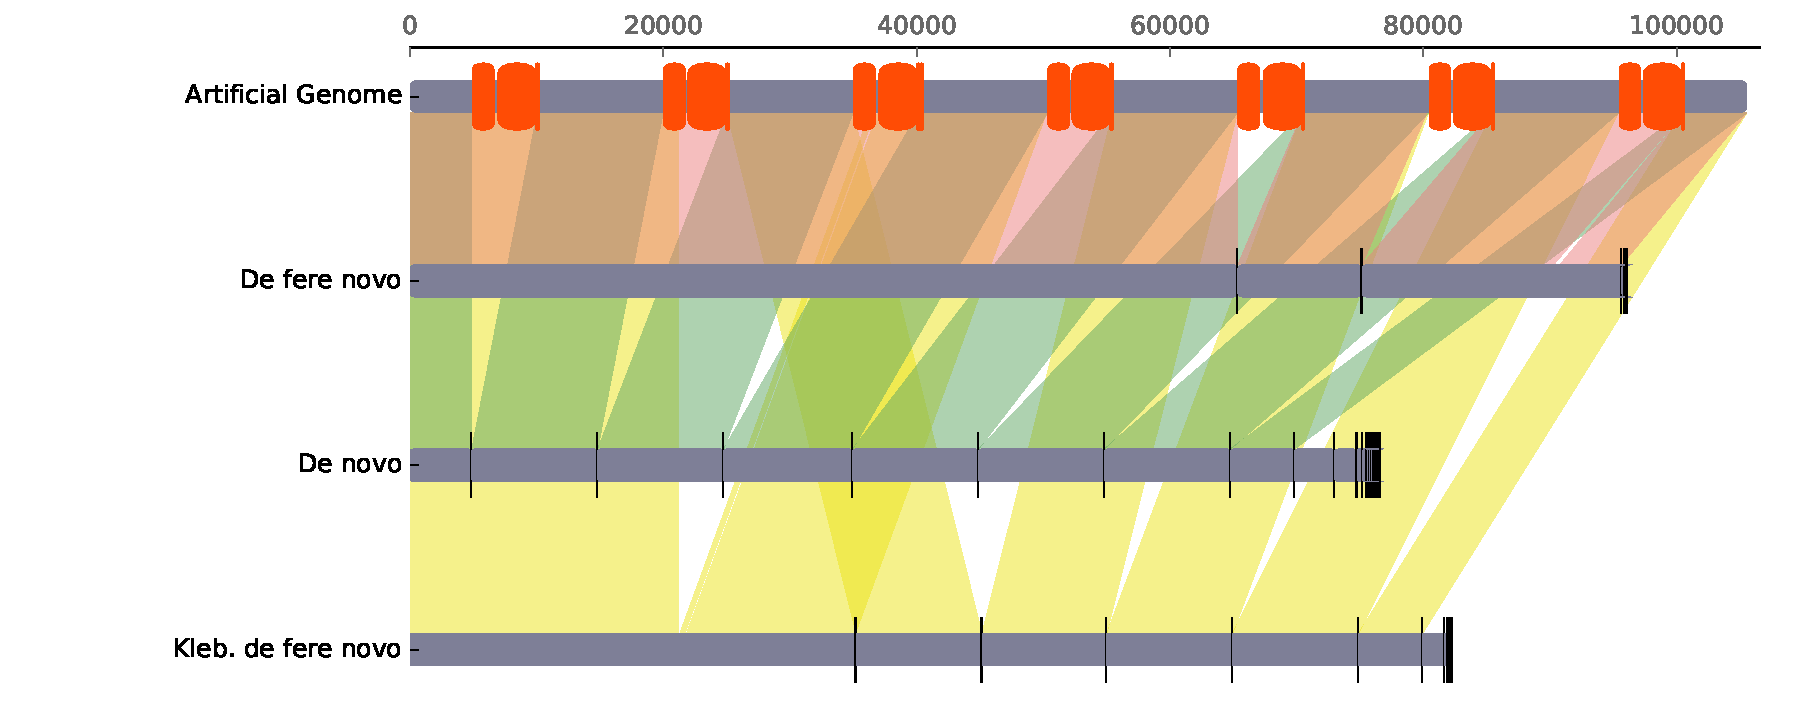
\includegraphics[width=1.25\textwidth]{~/GitHub/FB/Ecoli_comparative_genomics/doc/presentations/MyNUIG(mnuigtheme)/frequentFigs/PrettyMauve.pdf}

  Failed to detect false positives
\end{frame}


\begin{frame}[fragile]
  \frametitle{Solution 2}
  \begin{itemize}
  \item Annotate rDNAs and extract just flanking regions from reference and assemblies
  \item Use BLAST to find best reciprocal matches
  \item Parse fragment pairs
  \end{itemize}
  \centering
  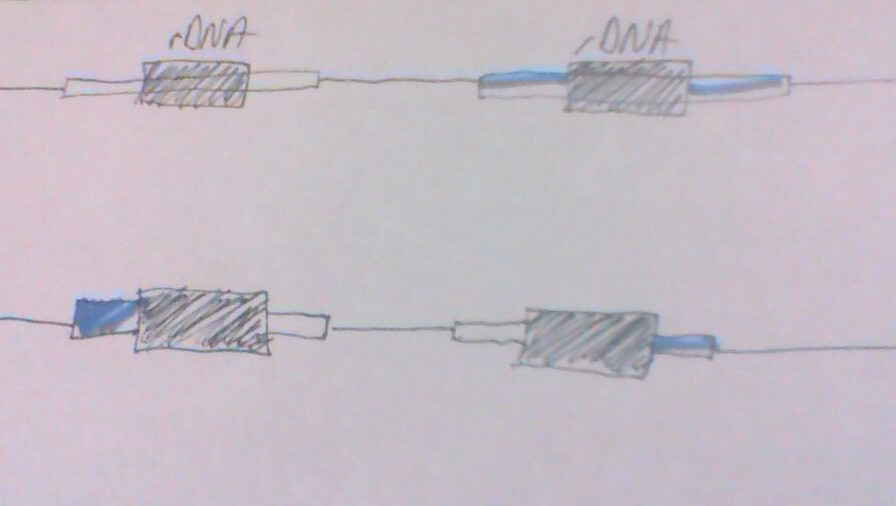
\includegraphics[width=1\textwidth]{~/GitHub/FB/Ecoli_comparative_genomics/doc/presentations/MyNUIG(mnuigtheme)/frequentFigs/misjoin}


\end{frame}

\begin{frame}[fragile]
  \frametitle{Solution 2: Results}
  Accurately characterized true positives
  Accurately detected false positives
\end{frame}

\begin{frame}[fragile]
  \frametitle{Work for the Week}
  \begin{itemize}
  \item Apply riboScore to all the results
  \item Determine effectiveness on real data
  \item Make a pipeline-specific version for automated error correction
  \end{itemize}
\end{frame}


% \plain{}{Questions?}

\end{document}
